\documentclass[acmsmall, nonacm, screen]{acmart} %sigconf

\def\BibTeX{{\rm B\kern-.05em{\sc i\kern-.025em b}\kern-.08emT\kern-.1667em\lower.7ex\hbox{E}\kern-.125emX}}
    
\copyrightyear{2019}
\acmYear{2019}
\acmMonth{04}

%\citestyle{acmauthoryear}
\usepackage{tikz}

\begin{document}

% The "title" command has an optional parameter, allowing the author to define a "short title" to be used in page headers.
\title{Towards Causality in Data Cleaning}

\author{Martin Gauch}
%\authornote{...}
\email{martin.gauch@uwaterloo.ca}
\affiliation{%
  \institution{University of Waterloo}
  \streetaddress{200 University Avenue West}
  \city{Waterloo}
  \state{ON}
  \postcode{N2L 3G1}
}

\begin{abstract}
abstract\\
\end{abstract}

%\keywords{data cleaning, causality, causal inference, observational study}

\maketitle

\section{Introduction}

\subsection{Problem Statement}

The notion of causality is not well-explored in the area of data cleaning. 
Existing solutions to analyze errors such as Data X-Ray \cite{Wang15} can identify possible causes for errors in a data set. They are however incapable to statistically justify the causal relationship. 
Instead, they return predicates that correlate with the errors, ranked according to a heuristic cost function. 
Hence, it remains unclear whether the reported reason truly caused the error or if there may be an unrecognized confounding factor.

\subsection{Challenges}
Finding and statistically justifying error causes in a data-driven way is challenging for several reasons. 
The amount of possible causes increases exponentially with the number of attributes and distinct values in a data set, which makes it computationally intractable to test every potential cause.\\

Further, even to test one single cause, we need to account for confounding factors. In a naive approach, such factors lead to exponentially increasing data requirements:
For each combination of con-founding factor values, we would need tuples that match the cause and tuples that don't. Similarly, larger factor domain spaces further exponentially increase the amount of required data.


\subsection{Contributions}
We explore ways to statistically approve or reject suspected causes for errors in a given erroneous data set.
We focus on the causal analysis and assume that errors are already flagged and the user has a suspicion about the error cause. 
This is a reasonable assumption as there exist tools for error detection as well as heuristic approaches to finding possible explanations. Often, common sense already suggests an error explanation that can be tested. Alternatively, there exist heuristics-based approaches to find possible explanations, e.g.\ Data X-Ray.\\

On synthetic and real-world data sets with known errors and hypothesized causes, we reformulate the hypothesis testing problem as causal analysis of an observational study \cite{Rosenbaum02}: We consider the proposed cause to be the treatment and the error to be the outcome.
In this observational study interpretation, we analyze the hypothesis of a causal relationship between treatment and outcome using causal inference methods. 
Such methods are well-known in other research areas such as medical sciences and have shown potential in their application to large data sets \cite{Robins16}.
If we find the treatment to significantly affect the outcome, this approves the hypothesized cause. In case there is no significant treatment effect, we reject the proposed explanation.\\

To account for confounding variables, we treat all further columns (i.e., all but treatment and outcome) as potential confounders. To reduce the amount of required data when accounting for confounders, we employ propensity score stratification \cite{Austin11}.\\

Finally, we investigate how these causal analysis tools can be employed to analyze bias in machine learning model predictions.\\


\section{Background}

\subsection{Observational Studies}
An observational study is an experimental setting in which researchers try to infer the effect of a \textit{treatment} on a specific \textit{outcome}.
In contrast to a randomized study, the independent variables are not under the researchers' control---they can only observe, not assign treatment.
This has a serious impact on how the collected data need to be interpreted. 
To account for possible bias in the treatment assignment, one needs to compare the outcome for similar treated and untreated individuals.
Additionally, one needs to control for \textit{confounding} variables that affect both the treatment assignment and the outcome.\\

Ideally, we would compare \textit{counterfactuals}: If we knew each individual's outcome under treatment \textit{and} non-treatment, holding all independent variables constant, we could easily calculate the treatment effect as the average difference in actual and counterfactual outcome.
In practice however, we do not know the counterfactual outcome, as we can only observe one treatment decision per individual.
Hence, causal analysis techniques for observational studies try to find and compare similar individuals among the treated and untreated populations and compare those.
One common approach for such comparisons is \textit{propensity score stratification}. Here, we train a simple machine learning model to predict each individual's \textit{propensity score}---its likelihood to be treated---given the independent variables.
The idea is that individuals with similar scores but different treatment are good candidates to be compared. 
Therefore, we partition the population into groups with similar propensity scores and calculate the treatment effect within each stratum as in \autoref{eq:ate}.
\begin{equation}
\label{eq:ate}
\begin{aligned}
\text{ATE} &= \mathbb{E}(O_{i1} | T=1) - \mathbb{E}(O_{i0} | T=0)\\
 &= \sum_{i=1}^{k}{\frac{1}{N_i}(\overline{O}_{i, T = 1} - \overline{O}_{i, T = 0})}
\end{aligned}
\end{equation}
Here, $O_{ij}$ is the outcome for an individual $i$ under treatment $T=j$, and $\overline{O}_{i, T = j}$ is the average outcome in stratum $i$ where treatment $T = j$, and $N_i$ is the size of stratum $i$.\\

Sometimes, we are not actually interested in the treatment effect among the whole population, but rather in the counterfactual outcome for the treated subpopulation. That is, we try to answer the question "How did the treatment affect the treated individuals?" In this case, we calculate the \textit{average treatment effect on the treated} as in \autoref{eq:att}.
\begin{equation}
\label{eq:att}
\begin{aligned}
\text{ATT} &= \mathbb{E}(O_{i1} | T=1) - \mathbb{E}(O_{i0} | T=1)\\
 &= \sum_{i=1}^{k}{\frac{1}{N_{i, T = 1}}(\overline{O}_{i,T = 1} - \overline{O}_{i,T = 0})}
\end{aligned}
\end{equation}
Here, $O_{i0}$ is the unobserved outcome for an individual $i$ had it not been treated, and $N_{i, T = 1}$ is the amount of treated individuals in stratum $i$.\\

While propensity score stratification is a powerful tool, there remain limitations to the analysis of observational study data. 
If the covariate distributions in a stratum's treated and untreated subpopulation are significantly different, we cannot draw any causal conclusions as we cannot be sure if we are missing confounding effects of this covariate.
We can test the distributions for similarity using $\chi^2$-hypothesis tests for categorical and Kolmogorov-Smirnov tests for continuous independent variables \cite{Sekhon08}.

\subsection{Causal Inference}

Propensity score stratification \cite{Austin11} is one of several common techniques used in observational studies that tries to reduce any bias introduced by confounding factors when available data is limited.\\

\subsection{Error Explanation}

.\\


\section{Related Work}
In the context of databases, Wang et al.\ use Bayesian analysis to help users finding reasons for errors in a data set \cite{Wang15}. 
Their framework uses a heuristic cost function that optimizes for conciseness, specificity and consistency. Further research focuses on explaining errors in database query output and either tries to fix the underlying data \cite{Wu13} or the query \cite{Tran10}.\\

The data mining community recently started researching the area of \textit{discrimination-aware data mining}, where analysts try to extract unbiased knowledge from potentially biased data sets. Bonchi et al.\ highlight bias in data sets using Bayesian probabilistic causal graphs \cite{Bonchi2017}. In a more machine-learning oriented setting, Zemel et al.\ create embeddings of data tuples that allow subsequent models to learn based on unbiased representations \cite{Zemel13}.\\

Causal inference is much more exhaustively researched in social and medical sciences. In these areas, scientists often need to test cause-effect hypotheses through observational studies, as randomized trials are not always ethically or physically feasible \cite{Rosenbaum02}.
With Big Data applications becoming increasingly ubiquitous, Hern\'{a}n et al.\ study to what extent we can approximate randomized experiments through using large sets of observational data \cite{Robins16}.
While clearly not every trial can be emulated through data analysis, they find that under reasonable assumptions it is possible to approximate randomization.\\


\section{Experiments}
We conduct experiments on both synthetic and real-world data sets, where we analyze the causal effect of an assumed error explanation.
We view the data sets as outcomes of an observational study, where the assumed cause is the treatment and a tuple's correctness is the outcome.
All further data set attributes are treated as covariates that might induce bias on the treatment assignment.
Consequently, we apply propensity score stratification to control for this bias.\\

In summary, each analysis consists of the following steps:
\begin{enumerate}
\item For a given data set with attributes $X = \{X_1, \dots, X_k\}$ and known erroneous tuples $t \in E$, find attribute-value combinations $X_i = x_i, \quad (i \in I)$ that are assumed to explain the errors.
\item Introduce a new binary treatment attribute $T$ where $t[T] = 1 \Leftrightarrow \forall i \in I: t[X_i] = x_i$.
\item Introduce a new binary outcome attribute $O$ where $t[O] = 1 \Leftrightarrow t \in E$.
\item Train a random forest classifier to predict $T$ given the independent variables $X \setminus \{X_i | i \in I\}$ and apply it to all tuples to obtain a propensity score for each individual.
\item Partition the data set into groups of similar propensity score.
\item In each partition, compare the covariate distributions of the treated with the untreated using $\chi^2$- or Kolmogorov-Smirnov tests of independence. If the independence tests cannot reject the hypothesis of identical distributions, we can continue.
\item\label{exp:ate} Calculate the average treatment effect:
\[
\text{ATE} = \sum_{i=1}^{k}{\frac{1}{N_i}(\overline{O}_{i, T = 1} - \overline{O}_{i, T = 0})}
\]
\item To provide a measure of significance, we compare the effect to a simulated placebo treatment. We assign $t[T]$ uniformly at random to $0$ or $1$ for all tuples and calculate the new treatment effect.
By repeating this process $m$ times, we obtain a sample $p = (p_1, \dots, p_m)$ of the placebo effect distribution.
\item If the observed treatment effect from step \ref{exp:ate} is outside the $95\%$-bounds of $p$, we can be reasonably certain that the observed effect is no coincidence.
\end{enumerate}

Note that there remain inherent limitations to the interpretability of observational studies. We have to assume \textit{ignorability}, i.e. that the data set's attributes $X$ include all confounding variables which might affect the outcome.
Unlike planned experimental studies, we cannot guarantee truly random treatment assignment. Nevertheless, a careful analysis of available data constitutes a step towards a more justifiable notion of error causality.\\

In the following sections, we describe the results of our experiments on synthetic and real-world data as well as the application of the observational study framework to estimate machine learning model bias.\\

\subsection{Synthetic Data Set}
We generate a data set in which we know the actual cause of errors. Modeling personal data records, it contains $10,000$ records with the columns shown in \autoref{tab:synth}. 
To simulate transcription errors, records representing people born in Asia are flagged as erroneous with probability $0.2$. Other records are flagged faulty with probability $0.05$ to simulate random errors.
Further, the attribute \textit{citizenship continent} is correlated with the actual error cause \textit{birth continent}.
\begin{table}[htbp]
\begin{center}
\begin{tabular}{ll}
\toprule 
Attribute & Number of distinct values \\ 
\midrule 
Source & $4$ \\ 
Last name  & randomly generated \\ 
Birth continent  & $3$ \\ 
Birth country  & $8$ \\ 
Citizenship continent  & $3$ \\ 
Citizenship country  & $8$ \\ 
Number of children & $4$ \\ 
Marital status & $4$ \\ 
\bottomrule 
\end{tabular} 
\caption{Synthetic data set attributes}
\label{tab:synth}
\end{center}
\end{table}
We apply Data X-Ray as an existing error explanation, which returns \{\textit{birth continent} = Asia\} and \{\textit{citizenship continent} = Asia\} as possible causes. Hence, we analyze both hypotheses in the observational study setting. \autoref{fig:causalGraph} shows the causal graph for the assumed cause \{\textit{birth continent} = Asia\}.\\
\begin{figure}[htbp]


\tikzset{every picture/.style={line width=0.75pt}} %set default line width to 0.75pt        

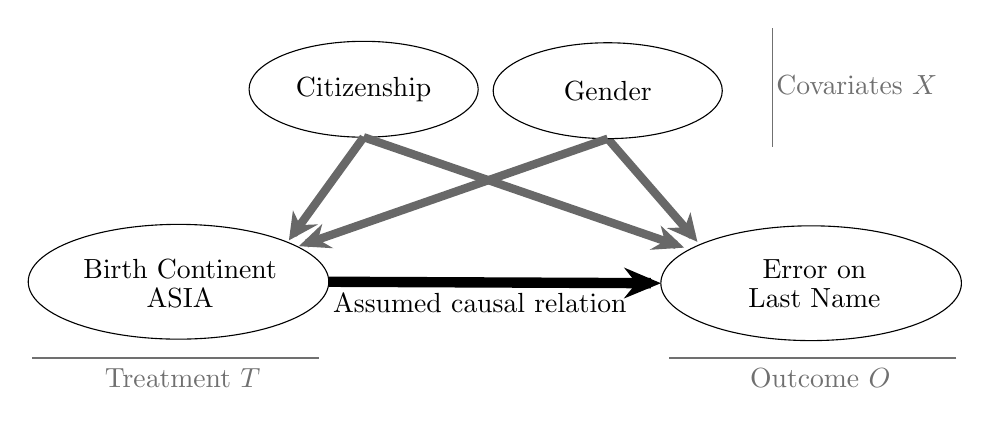
\begin{tikzpicture}[x=0.75pt,y=0.75pt,yscale=-0.7,xscale=0.8]
%uncomment if require: \path (0,300); %set diagram left start at 0, and has height of 300

%Shape: Ellipse [id:dp01555367087711701] 
\draw   (81,203.5) .. controls (81,181.68) and (121.52,164) .. (171.5,164) .. controls (221.48,164) and (262,181.68) .. (262,203.5) .. controls (262,225.32) and (221.48,243) .. (171.5,243) .. controls (121.52,243) and (81,225.32) .. (81,203.5) -- cycle ;
%Shape: Ellipse [id:dp5483766550069732] 
\draw   (462,204.5) .. controls (462,182.68) and (502.52,165) .. (552.5,165) .. controls (602.48,165) and (643,182.68) .. (643,204.5) .. controls (643,226.32) and (602.48,244) .. (552.5,244) .. controls (502.52,244) and (462,226.32) .. (462,204.5) -- cycle ;
%Straight Lines [id:da1339514120696047] 
\draw [color={rgb, 255:red, 0; green, 0; blue, 0 }  ,draw opacity=1 ][line width=3.75]    (262,203.5) -- (456,204.47) ;
\draw [shift={(462,204.5)}, rotate = 180.29] [fill={rgb, 255:red, 0; green, 0; blue, 0 }  ,fill opacity=1 ][line width=3.75]  [draw opacity=0] (22.33,-10.72) -- (0,0) -- (22.33,10.73) -- (14.83,0) -- cycle    ;

%Shape: Ellipse [id:dp9243404607646779] 
\draw  [fill={rgb, 255:red, 255; green, 255; blue, 255 }  ,fill opacity=1 ] (214,71) .. controls (214,52.77) and (244.89,38) .. (283,38) .. controls (321.11,38) and (352,52.77) .. (352,71) .. controls (352,89.23) and (321.11,104) .. (283,104) .. controls (244.89,104) and (214,89.23) .. (214,71) -- cycle ;
%Straight Lines [id:da47301284684960065] 
\draw [color={rgb, 255:red, 104; green, 104; blue, 104 }  ,draw opacity=1 ][line width=3]    (430,105) -- (480.97,172.02) ;
\draw [shift={(484,176)}, rotate = 232.74] [fill={rgb, 255:red, 104; green, 104; blue, 104 }  ,fill opacity=1 ][line width=3]  [draw opacity=0] (18.75,-9.01) -- (0,0) -- (18.75,9.01) -- (12.45,0) -- cycle    ;

%Shape: Ellipse [id:dp5825215913753231] 
\draw  [fill={rgb, 255:red, 255; green, 255; blue, 255 }  ,fill opacity=1 ] (361,72) .. controls (361,53.77) and (391.89,39) .. (430,39) .. controls (468.11,39) and (499,53.77) .. (499,72) .. controls (499,90.23) and (468.11,105) .. (430,105) .. controls (391.89,105) and (361,90.23) .. (361,72) -- cycle ;
%Straight Lines [id:da34453571650557135] 
\draw [color={rgb, 255:red, 104; green, 104; blue, 104 }  ,draw opacity=1 ][line width=3]    (283,104) -- (471.35,178.17) ;
\draw [shift={(476,180)}, rotate = 201.49] [fill={rgb, 255:red, 104; green, 104; blue, 104 }  ,fill opacity=1 ][line width=3]  [draw opacity=0] (18.75,-9.01) -- (0,0) -- (18.75,9.01) -- (12.45,0) -- cycle    ;

%Straight Lines [id:da8978058209783277] 
\draw [color={rgb, 255:red, 104; green, 104; blue, 104 }  ,draw opacity=1 ][line width=3]    (430,105) -- (248.65,177.15) ;
\draw [shift={(244,179)}, rotate = 338.3] [fill={rgb, 255:red, 104; green, 104; blue, 104 }  ,fill opacity=1 ][line width=3]  [draw opacity=0] (18.75,-9.01) -- (0,0) -- (18.75,9.01) -- (12.45,0) -- cycle    ;

%Straight Lines [id:da17001230828023528] 
\draw [color={rgb, 255:red, 104; green, 104; blue, 104 }  ,draw opacity=1 ][line width=3]    (283,104) -- (240.68,170.78) ;
\draw [shift={(238,175)}, rotate = 302.37] [fill={rgb, 255:red, 104; green, 104; blue, 104 }  ,fill opacity=1 ][line width=3]  [draw opacity=0] (18.75,-9.01) -- (0,0) -- (18.75,9.01) -- (12.45,0) -- cycle    ;

%Straight Lines [id:da5757713157103644] 
\draw [color={rgb, 255:red, 112; green, 112; blue, 112 }  ,draw opacity=1 ]   (529,29) -- (529,111) ;


%Straight Lines [id:da8098889471290196] 
\draw [color={rgb, 255:red, 112; green, 112; blue, 112 }  ,draw opacity=1 ]   (256,256) -- (83,256) ;


%Straight Lines [id:da9998346743193436] 
\draw [color={rgb, 255:red, 112; green, 112; blue, 112 }  ,draw opacity=1 ]   (640,256) -- (467,256) ;



% Text Node
\draw (172.5,194.5) node  [align=left] {Birth Continent};
% Text Node
\draw (172.5,214.5) node  [align=left] {ASIA};
% Text Node
\draw (554.5,194.5) node  [align=left] {Error on};
% Text Node
\draw (554.5,214.5) node  [align=left] {Last Name};
% Text Node
\draw (283,71) node  [align=left] {Citizenship};
% Text Node
\draw (430,72) node  [align=left] {Gender};
% Text Node
\draw (353,218) node  [align=left] {Assumed causal relation};
% Text Node
\draw (580,68) node [color={rgb, 255:red, 112; green, 112; blue, 112 }  ,opacity=1 ] [align=left] {Covariates $\displaystyle X$};
% Text Node
\draw (174,270) node [color={rgb, 255:red, 112; green, 112; blue, 112 }  ,opacity=1 ] [align=left] {Treatment $\displaystyle T$};
% Text Node
\draw (558,270) node [color={rgb, 255:red, 112; green, 112; blue, 112 }  ,opacity=1 ] [align=left] {Outcome $\displaystyle O$};


\end{tikzpicture}

\caption{Assumed causal graph for the error explanation \{\textit{birth continent} = Asia\}.}
\label{fig:causalGraph}
\end{figure}

By analyzing causality in a statistical way, we can correctly distinguish actual cause and correlated covariate. The average treatment effect among the treated for \textit{birth continent} is $-0.14$, while the treatment effect for \textit{citizenship continent} of $-0.01$ is within the $95\%$-bounds of placebo treatment effect.
Consequently, we can reject \textit{citizenship continent} and approve \textit{birth continent} as a cause for the errors in the data set.
In the empirical quantile-quantile plot in \autoref{fig:qqBirth} we repeatedly analyze subsamples of the data set to obtain a distribution of treatment effects that we compare against placebo effect.
The plot clearly shows the difference between the two distributions, which further emphasizes the causal relationship.
\begin{figure}[htbp]
\includegraphics[width=0.6\linewidth]{figures/qqBirth.pdf}
\caption{Empirical quantile-quantile plot showing the difference between placebo and actual treatment (\textit{birth continent} = Asia) effect on erroneous outcomes.}
\label{fig:qqBirth}
\end{figure}


\subsection{Real-World Data Sets}
To find out to which extent causal analysis is possible in practice, we try to explain errors in two existing real-world data sets, the Intel Lab sensor data set\footnote{\url{http://db.csail.mit.edu/labdata/labdata.html}} and knowledge extraction tuples from the \textit{Reverb} system\footnote{\url{http://reverb.cs.washington.edu/}}. 
The knowledge extraction tuples are already labeled as correct or incorrect, so we consider incorrect extractions as errors. As the space of possible causes, we use the extracted statement's part-of-speech tags. For the sensor data, we consider \textit{NA}-values of light measurements as errors.\\

Again, we apply Data X-Ray to obtain possible causes. We find that is is quite hard to fine-tune the model parameters such that the result set is neither empty nor merely listing all tuples that contain errors.
Also, Data X-Ray's run time quickly gets intractable when categorical attributes have large domains or numerical attributes are involved.
This is another advantage of our analysis approach: The propensity-score based statistical analysis can make use of continuous attributes and attributes with large domain spaces without increasing complexity.\\

With the given data sets however, we are unable to reach a definitive conclusion about the error causes.
The reason for this is that there are too many correlated covariates, such that the covariate distributions of treated and untreated tuples are not balanced enough within some propensity score strata.
Further, usually the assumed cause does not explain all errors. Hence, the treated subpopulation with positive outcome, i.e.\ the erroneous tuples that match the assumed cause, is relatively small. 
Even in the large sensor data set with more than two million tuples, only about $9,400$ tuples have NA-values for their light measurement. Out of these, only a subset matches any non-trivial error cause such as low voltage.
In consequence, it is impossible to approve or reject an explanation in a significant way.

\subsection{Estimating Machine Learning Model Bias}
Another interesting area where we can apply our approach of causal analysis is estimating bias of machine learning models.
As an example, we use the US Census data set and train a random forest classifier to predict peoples' income as above or below $\$50,000$\footnote{\url{https://archive.ics.uci.edu/ml/datasets/Census+Income}}.
Next, we try to find out whether the classifier is biased regarding the attribute \textit{gender}, i.e.\ whether it is more likely to predict low income for female than for male individuals.
A challenge in this analysis is that one cannot naively use the training or test data to evaluate the bias, as those data sets probably are biased, too---after all, this is where the model bias comes from.\\

To solve this problem, we realize that for a simple analysis we do not actually need ground truth labels. 
Hence, we can generate random tuples with \textit{gender} taking values male and female equally often. We can then apply the classifier and obtain predicted incomes. 
Now we consider the value of \textit{gender} as the treatment, and the income classification as the outcome, which enables us to estimate the treatment effect.
With the given random forest classifier that achieves a classification accuracy of $0.86$, we find an average treatment effect of $-0.05$, which is well outside the $95\%$-bounds of placebo treatment.
The empirical quantile-quantile plot reflects this and shows the actual treatment to differ significantly from placebo treatment, as \autoref{fig:qqML} shows.
This result suggests that the classifier is in fact biased towards lower incomes for female individuals.\\

\begin{figure}[htbp]
\includegraphics[width=0.6\linewidth]{figures/qqML.pdf}
\caption{Empirical quantile-quantile plot showing the difference between placebo and actual treatment (\textit{gender} = female) effect on income prediction.}
\label{fig:qqML}
\end{figure}

The approach of generating random unlabeled data has the major advantage that we are able to produce as much data as needed for a statistically significant analysis.
We also tried to analyze the bias based on the actual test data by viewing gender as the treatment and falsely predicted low income as the outcome. 
In this case however, we need to account for covariates in the data set as these might be potentially confounding.
As with the analysis of real-world data in the previous section, this covariate-accounting heavily increases data requirements, rendering a statistically significant analysis impossible with the available data.


\section{Conclusion and Future Work}

Sometimes, the user might even be in control over the data generation process. 
If so, we can ask for additional data tuples that would help the causal inference. Especially, users can supply tuples that allow estimating the counterfactual outcome.\\


%\begin{acks}
%\end{acks}

\bibliographystyle{ACM-Reference-Format}
\bibliography{report}

%\appendix

\end{document}
